% Options for packages loaded elsewhere
\PassOptionsToPackage{unicode}{hyperref}
\PassOptionsToPackage{hyphens}{url}
\PassOptionsToPackage{dvipsnames,svgnames,x11names}{xcolor}
%
\documentclass[
  letterpaper,
  DIV=11,
  numbers=noendperiod]{scrartcl}

\usepackage{amsmath,amssymb}
\usepackage{lmodern}
\usepackage{iftex}
\ifPDFTeX
  \usepackage[T1]{fontenc}
  \usepackage[utf8]{inputenc}
  \usepackage{textcomp} % provide euro and other symbols
\else % if luatex or xetex
  \usepackage{unicode-math}
  \defaultfontfeatures{Scale=MatchLowercase}
  \defaultfontfeatures[\rmfamily]{Ligatures=TeX,Scale=1}
\fi
% Use upquote if available, for straight quotes in verbatim environments
\IfFileExists{upquote.sty}{\usepackage{upquote}}{}
\IfFileExists{microtype.sty}{% use microtype if available
  \usepackage[]{microtype}
  \UseMicrotypeSet[protrusion]{basicmath} % disable protrusion for tt fonts
}{}
\makeatletter
\@ifundefined{KOMAClassName}{% if non-KOMA class
  \IfFileExists{parskip.sty}{%
    \usepackage{parskip}
  }{% else
    \setlength{\parindent}{0pt}
    \setlength{\parskip}{6pt plus 2pt minus 1pt}}
}{% if KOMA class
  \KOMAoptions{parskip=half}}
\makeatother
\usepackage{xcolor}
\setlength{\emergencystretch}{3em} % prevent overfull lines
\setcounter{secnumdepth}{-\maxdimen} % remove section numbering
% Make \paragraph and \subparagraph free-standing
\ifx\paragraph\undefined\else
  \let\oldparagraph\paragraph
  \renewcommand{\paragraph}[1]{\oldparagraph{#1}\mbox{}}
\fi
\ifx\subparagraph\undefined\else
  \let\oldsubparagraph\subparagraph
  \renewcommand{\subparagraph}[1]{\oldsubparagraph{#1}\mbox{}}
\fi

\usepackage{color}
\usepackage{fancyvrb}
\newcommand{\VerbBar}{|}
\newcommand{\VERB}{\Verb[commandchars=\\\{\}]}
\DefineVerbatimEnvironment{Highlighting}{Verbatim}{commandchars=\\\{\}}
% Add ',fontsize=\small' for more characters per line
\usepackage{framed}
\definecolor{shadecolor}{RGB}{241,243,245}
\newenvironment{Shaded}{\begin{snugshade}}{\end{snugshade}}
\newcommand{\AlertTok}[1]{\textcolor[rgb]{0.68,0.00,0.00}{#1}}
\newcommand{\AnnotationTok}[1]{\textcolor[rgb]{0.37,0.37,0.37}{#1}}
\newcommand{\AttributeTok}[1]{\textcolor[rgb]{0.40,0.45,0.13}{#1}}
\newcommand{\BaseNTok}[1]{\textcolor[rgb]{0.68,0.00,0.00}{#1}}
\newcommand{\BuiltInTok}[1]{\textcolor[rgb]{0.00,0.23,0.31}{#1}}
\newcommand{\CharTok}[1]{\textcolor[rgb]{0.13,0.47,0.30}{#1}}
\newcommand{\CommentTok}[1]{\textcolor[rgb]{0.37,0.37,0.37}{#1}}
\newcommand{\CommentVarTok}[1]{\textcolor[rgb]{0.37,0.37,0.37}{\textit{#1}}}
\newcommand{\ConstantTok}[1]{\textcolor[rgb]{0.56,0.35,0.01}{#1}}
\newcommand{\ControlFlowTok}[1]{\textcolor[rgb]{0.00,0.23,0.31}{#1}}
\newcommand{\DataTypeTok}[1]{\textcolor[rgb]{0.68,0.00,0.00}{#1}}
\newcommand{\DecValTok}[1]{\textcolor[rgb]{0.68,0.00,0.00}{#1}}
\newcommand{\DocumentationTok}[1]{\textcolor[rgb]{0.37,0.37,0.37}{\textit{#1}}}
\newcommand{\ErrorTok}[1]{\textcolor[rgb]{0.68,0.00,0.00}{#1}}
\newcommand{\ExtensionTok}[1]{\textcolor[rgb]{0.00,0.23,0.31}{#1}}
\newcommand{\FloatTok}[1]{\textcolor[rgb]{0.68,0.00,0.00}{#1}}
\newcommand{\FunctionTok}[1]{\textcolor[rgb]{0.28,0.35,0.67}{#1}}
\newcommand{\ImportTok}[1]{\textcolor[rgb]{0.00,0.46,0.62}{#1}}
\newcommand{\InformationTok}[1]{\textcolor[rgb]{0.37,0.37,0.37}{#1}}
\newcommand{\KeywordTok}[1]{\textcolor[rgb]{0.00,0.23,0.31}{#1}}
\newcommand{\NormalTok}[1]{\textcolor[rgb]{0.00,0.23,0.31}{#1}}
\newcommand{\OperatorTok}[1]{\textcolor[rgb]{0.37,0.37,0.37}{#1}}
\newcommand{\OtherTok}[1]{\textcolor[rgb]{0.00,0.23,0.31}{#1}}
\newcommand{\PreprocessorTok}[1]{\textcolor[rgb]{0.68,0.00,0.00}{#1}}
\newcommand{\RegionMarkerTok}[1]{\textcolor[rgb]{0.00,0.23,0.31}{#1}}
\newcommand{\SpecialCharTok}[1]{\textcolor[rgb]{0.37,0.37,0.37}{#1}}
\newcommand{\SpecialStringTok}[1]{\textcolor[rgb]{0.13,0.47,0.30}{#1}}
\newcommand{\StringTok}[1]{\textcolor[rgb]{0.13,0.47,0.30}{#1}}
\newcommand{\VariableTok}[1]{\textcolor[rgb]{0.07,0.07,0.07}{#1}}
\newcommand{\VerbatimStringTok}[1]{\textcolor[rgb]{0.13,0.47,0.30}{#1}}
\newcommand{\WarningTok}[1]{\textcolor[rgb]{0.37,0.37,0.37}{\textit{#1}}}

\providecommand{\tightlist}{%
  \setlength{\itemsep}{0pt}\setlength{\parskip}{0pt}}\usepackage{longtable,booktabs,array}
\usepackage{calc} % for calculating minipage widths
% Correct order of tables after \paragraph or \subparagraph
\usepackage{etoolbox}
\makeatletter
\patchcmd\longtable{\par}{\if@noskipsec\mbox{}\fi\par}{}{}
\makeatother
% Allow footnotes in longtable head/foot
\IfFileExists{footnotehyper.sty}{\usepackage{footnotehyper}}{\usepackage{footnote}}
\makesavenoteenv{longtable}
\usepackage{graphicx}
\makeatletter
\def\maxwidth{\ifdim\Gin@nat@width>\linewidth\linewidth\else\Gin@nat@width\fi}
\def\maxheight{\ifdim\Gin@nat@height>\textheight\textheight\else\Gin@nat@height\fi}
\makeatother
% Scale images if necessary, so that they will not overflow the page
% margins by default, and it is still possible to overwrite the defaults
% using explicit options in \includegraphics[width, height, ...]{}
\setkeys{Gin}{width=\maxwidth,height=\maxheight,keepaspectratio}
% Set default figure placement to htbp
\makeatletter
\def\fps@figure{htbp}
\makeatother

\KOMAoption{captions}{tableheading}
\makeatletter
\makeatother
\makeatletter
\makeatother
\makeatletter
\@ifpackageloaded{caption}{}{\usepackage{caption}}
\AtBeginDocument{%
\ifdefined\contentsname
  \renewcommand*\contentsname{Table of contents}
\else
  \newcommand\contentsname{Table of contents}
\fi
\ifdefined\listfigurename
  \renewcommand*\listfigurename{List of Figures}
\else
  \newcommand\listfigurename{List of Figures}
\fi
\ifdefined\listtablename
  \renewcommand*\listtablename{List of Tables}
\else
  \newcommand\listtablename{List of Tables}
\fi
\ifdefined\figurename
  \renewcommand*\figurename{Figure}
\else
  \newcommand\figurename{Figure}
\fi
\ifdefined\tablename
  \renewcommand*\tablename{Table}
\else
  \newcommand\tablename{Table}
\fi
}
\@ifpackageloaded{float}{}{\usepackage{float}}
\floatstyle{ruled}
\@ifundefined{c@chapter}{\newfloat{codelisting}{h}{lop}}{\newfloat{codelisting}{h}{lop}[chapter]}
\floatname{codelisting}{Listing}
\newcommand*\listoflistings{\listof{codelisting}{List of Listings}}
\makeatother
\makeatletter
\@ifpackageloaded{caption}{}{\usepackage{caption}}
\@ifpackageloaded{subcaption}{}{\usepackage{subcaption}}
\makeatother
\makeatletter
\@ifpackageloaded{tcolorbox}{}{\usepackage[many]{tcolorbox}}
\makeatother
\makeatletter
\@ifundefined{shadecolor}{\definecolor{shadecolor}{rgb}{.97, .97, .97}}
\makeatother
\makeatletter
\makeatother
\ifLuaTeX
  \usepackage{selnolig}  % disable illegal ligatures
\fi
\IfFileExists{bookmark.sty}{\usepackage{bookmark}}{\usepackage{hyperref}}
\IfFileExists{xurl.sty}{\usepackage{xurl}}{} % add URL line breaks if available
\urlstyle{same} % disable monospaced font for URLs
\hypersetup{
  pdftitle={Activity 4: Diving Penguins},
  colorlinks=true,
  linkcolor={blue},
  filecolor={Maroon},
  citecolor={Blue},
  urlcolor={Blue},
  pdfcreator={LaTeX via pandoc}}

\title{Activity 4: Diving Penguins}
\author{}
\date{10/10/2022}

\begin{document}
\maketitle
\ifdefined\Shaded\renewenvironment{Shaded}{\begin{tcolorbox}[enhanced, borderline west={3pt}{0pt}{shadecolor}, interior hidden, breakable, frame hidden, sharp corners, boxrule=0pt]}{\end{tcolorbox}}\fi

\hypertarget{terminology-review}{%
\section{Terminology review}\label{terminology-review}}

In today's activity, we will use simulation-based methods for conducting
a hypothesis test for a linear regression slope or correlation. Some
terms covered in this activity are:

\begin{itemize}
\tightlist
\item
  Correlation
\item
  Slope
\item
  Regression line
\end{itemize}

\hypertarget{diving-penguins}{%
\section{Diving Penguins}\label{diving-penguins}}

Emperor penguins are the most accomplished divers among birds, making
routine dives of 5--12 minutes, with the longest recorded dive over 27
minutes. These birds can also dive to depths of over 500 meters! Since
air-breathing animals like penguins must hold their breath while
submerged, the duration of any given dive depends on how much oxygen is
in the bird's body at the beginning of the dive, how quickly that oxygen
gets used, and the lowest level of oxygen the bird can tolerate. The
rate of oxygen depletion is primarily determined by the penguin's heart
rate. Consequently, studies of heart rates during dives can help us
understand how these animals regulate their oxygen consumption in order
to make such impressive dives.

In this study, the researchers equipped emperor penguins with devices
that record their heart rates during dives. The data set reports Dive
Heart Rate (beats per minute), the Duration (minutes) of dives, and
other related variables. Is there an association between dive heart rate
and the duration of the dive?

\begin{Shaded}
\begin{Highlighting}[]
\NormalTok{diving }\OtherTok{\textless{}{-}} \FunctionTok{read\_csv}\NormalTok{(}\StringTok{"Diving\_Penguins.csv"}\NormalTok{)}
\end{Highlighting}
\end{Shaded}

\begin{verbatim}
Rows: 125 Columns: 4
-- Column specification --------------------------------------------------------
Delimiter: ","
chr (1): Bird
dbl (3): Dive_HeartRate, Depth, Duration

i Use `spec()` to retrieve the full column specification for this data.
i Specify the column types or set `show_col_types = FALSE` to quiet this message.
\end{verbatim}

\begin{Shaded}
\begin{Highlighting}[]
\FunctionTok{head}\NormalTok{(diving)}
\end{Highlighting}
\end{Shaded}

\begin{verbatim}
# A tibble: 6 x 4
  Dive_HeartRate Depth Duration Bird 
           <dbl> <dbl>    <dbl> <chr>
1           88.8   5       1.05 EP19 
2          103.    9       1.18 EP19 
3           97.4  22       1.92 EP19 
4           85.3  25.5     3.47 EP19 
5           60.6  30.5     7.08 EP19 
6           77.6  32.5     4.77 EP19 
\end{verbatim}

\hypertarget{vocabulary-review}{%
\subsection{Vocabulary review}\label{vocabulary-review}}

\textbf{1. In this study, which variable will be on the \(x\)-axis? Is
it the response variable or the explanatory variable? Is it quantitative
or categorical?}

\key{The penguin's heart rate - $\text{Dive}\_\text{HeartRate}$ - will be on the $x$-axis as the explanatory variable for the study. This is quantitative (beats per minute).}

\vspace{1cm}

\textbf{2. Which variable is on the \(y\)-axis? Is it the response
variable or the explanatory variable? Is it quantitative or
categorical?}

\key{The duration of the penguin's dive - Duration - will be on the $y$-axis as the response variable for the study. This is quantitative (minutes).}

\vspace{1cm}

\textbf{3. How is this study different from other studies we have
considered?} \emph{(Hint: consider the number and types of variables.)}

\key{We now have two quantiative variables rather than one quantative variable.}

\vspace{.5in}

\hypertarget{exploratory-data-analysis}{%
\section{Exploratory Data Analysis}\label{exploratory-data-analysis}}

\hypertarget{visualizing-the-relationship---scatterplot}{%
\subsection{Visualizing the Relationship -
Scatterplot}\label{visualizing-the-relationship---scatterplot}}

A \emph{scatterplot} is a graph showing a dot for each observational
unit, where the location of the dot indicates the values of the
observational unit for both the explanatory and response variables.
Typically, the explanatory variable is placed on the \(x\)-axis and the
response variable is placed on the \(y\)-axis.

When describing a relationship or association between two quantitative
variables as seen through a scatterplot, we look for three aspects of
association: form, direction, and strength.

\begin{itemize}
\item
  The \textbf{form} of association between two quantitative variables is
  described by indicating whether a line would do a reasonable job
  summarizing the overall pattern in the data or if a curve would be
  better. It is important to note that, especially when the sample size
  is small, you don't want to let one or two points on the scatterplot
  change your interpretation of whether or not the form of association
  is linear. In general, assume that the form is linear unless there is
  compelling (strong) evidence in the scatterplot that the form is not
  linear.
\item
  The \textbf{direction} of association between two quantitative
  variables is either positive or negative, depending on whether or not
  the response variable (\texttt{Duration}) tends to increase (positive
  association) or decrease (negative association) as the explanatory
  variable (\texttt{Dive\_HeartRate}) increases.
\item
  In describing the \textbf{strength} of association revealed in a
  scatterplot, we see how closely the points follow a straight line or
  curve. If all the points fall pretty close to this straight line or
  curve, we say the association is strong. Weak associations will show
  little pattern in the scatterplot, and moderate associations will be
  somewhere in the middle.
\item
  When exploring the relationship and describing a scatterplot which
  visualizes two quantitative variables, we look for \textbf{unusual
  observations} or apparent \textbf{outliers}. Points which fall far
  from the trend of other points have the potential to be high leverage
  or high influential points.
\end{itemize}

\begin{figure}

{\centering 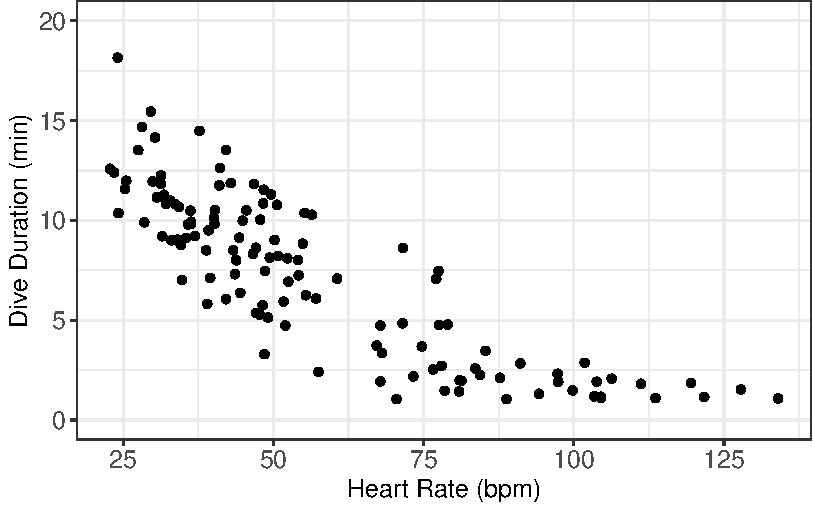
\includegraphics[width=0.7\textwidth,height=\textheight]{activity4-diving-penguins-key_files/figure-pdf/eda-1.pdf}

}

\end{figure}

\textbf{4. Describe the association between the variables as revealed in
the scatterplot above.} \emph{(Hint: Remember to comment on direction,
strength, and form of association as well as unusual observations. Also,
make sure you use the context of the study)}

\begin{itemize}
\item
  \key{Direction: Negative association (as Heart Rate increases, the Duration of the dive decreases).}
\item
  \key{Strength: There is a strong relationship between heart rate and duration as indicated by the obvious trend in the data.}
\item
  \key{Form: The association between heart rate and duration is close to linearly related (can reasonably fit a straight line through the set of points).}
\item
  \key{Unusual Observations/Outliers: Most points fall within the general trend, but there are a few penguin's with heart rates around 75 bpm that have a little higher dive durations than the rest. We have only a couple observations where the penguin's heart rate was above 125 bpm.}
\end{itemize}

\hypertarget{summarizing-the-relationship---correlation}{%
\subsection{Summarizing the Relationship -
Correlation}\label{summarizing-the-relationship---correlation}}

Describing the direction, form, and strength of association based on a
scatterplot, along with investigating unusual observations, is an
important first step in summarizing the relationship between two
quantitative variables. Another approach is to use a summary statistic.
One of the statistics most commonly used for this purpose is the
\textbf{correlation coefficient}. When the relationship has a roughly
linear form, it's strength and direction can be quantified by the
correlation.

The sample correlation coefficient, denoted \(r\), is a single number
that takes a value between -1 and 1, inclusive. Negative values of \(r\)
indicate a negative association, whereas positive values of \(r\)
indicate a positive association. It is important to note that the
correlation coefficient within a population is denoted \(\rho\) and
\(r\) is an estimate of \(\rho\).

\vspace{0.5cm}

\fbox{\begin{minipage}{45em}
\textbf{\large{Key Idea}} \\
The correlation coefficient is only applicable for data which has a linear form; non-linear data is not summarized well by the correlation coefficient. In fact, we could say that the correlation coefficient is a numerical summary of the \textbf{strength} and \textbf{direction} of a linear association between two quantitative variables.
\end{minipage}}

\hypertarget{some-key-ideas-to-remember}{%
\subsection{Some key ideas to
remember}\label{some-key-ideas-to-remember}}

\begin{itemize}
\tightlist
\item
  Correlation measures the relationship between a pair of variables; the
  correlation is the same regardless of which one is explanatory and
  which is response. \emph{(Be careful, the same is not true for
  regression coefficients!)}
\item
  Correlation is a number without units. It is not a percent!
\item
  The stronger the linear association is between the two variables, the
  closer the value of the correlation coefficient will be to either -1
  or 1, whereas weaker linear associations will have correlation
  coefficient values closer to 0. Moderate linear associations will
  typically have correlation coefficients in the range of 0.3 to 0.7, or
  -0.3 to -0.7.
\item
  Correlation can be sensitive to outliers and extreme values of either
  variable.
\end{itemize}

\hypertarget{calculating-the-correlation}{%
\subsection{Calculating the
Correlation}\label{calculating-the-correlation}}

The correlation coefficient uses a rather complex formula that is rarely
computed by hand; instead, people almost always use a calculator or
computer to calculate the value of the correlation coefficient. We will
use the \textbf{moderndive} \texttt{R} package to obtain the correlation
between two numerical variables. Specifically, we will use the
\texttt{get\_correlation()} function to obtain our sample correlation
coefficient.

The code will always look something like this:

\begin{verbatim}
get_correlation(data = <NAME OF DATASET>, 
                <Y-VARIABLE> ~ <X-VARIABLE>)
\end{verbatim}

You will be responsible for (1) filling in the name of the data set and
(2) filling in the names of the \(x\)-variable and \(y\)-variable.

I've filled in the code for you to obtain our sample correlation

\begin{Shaded}
\begin{Highlighting}[]
\FunctionTok{get\_correlation}\NormalTok{(}\AttributeTok{data =}\NormalTok{ diving, }
\NormalTok{                Duration }\SpecialCharTok{\textasciitilde{}}\NormalTok{ Dive\_HeartRate)}
\end{Highlighting}
\end{Shaded}

\begin{verbatim}
# A tibble: 1 x 1
     cor
   <dbl>
1 -0.846
\end{verbatim}

\textbf{5. Interpret the correlation obtained. Is it positive or
negative? What does this imply about the relationship between the
variables? Is it strong, moderate, or weak? How does this connect to
what you saw in the scatterplot?}

\key{A correlation coefficient of $r = -0.84$ tells us we have a strong negative association between a penguin's heart rate (bpm) and the duration of their dive (mins). This connects to our scatterplot because we can see the points follow a fairly apparent downward trend.}

\textbf{6. Say you had another observation at (100, 15), as in a penguin
with a heart rate of 100 beats per minute who dove for 15 minutes. How
do you think this would change the correlation coefficient?}

\key{The absolute value of the correlation coefficient would become smaller (i.e. closer to zero) because the point does not follow the strong trend.}

\hypertarget{least-squares-regression}{%
\section{Least Squares Regression}\label{least-squares-regression}}

\textbf{7. If you knew the heart rate of a penguin, what might be a way
to determine how long you would expect for them to dive for based on the
data?}

\key{With tools we previously learned, we could take the average of dive time for penguins with that heart rate from the data set. What we essentially do is find a line that goes through the center of the points as best as possible and call that line our "predicted" dive duration across the range of heart rates.}

\vspace{0.5cm}

Correlation measures strength of the association between two
quantitative variables when the sample data points tend to follow a
straight line. A natural question is then: what line do the points tend
to follow?

\vspace{0.5cm}

\textbf{8. Based on the scatterplot, would you say that a straight line
could summarize the relationship between dive duration and heart rate
reasonably well?}

\key{Yes, the trend is reasonably linear/straight.}

\vspace{0.5cm}

\textbf{9. Using the scatterplot below, draw the line you believe fits
the data the best. How did you decide where to draw your line? Is your
line the same as your group members?}

\begin{figure}

{\centering 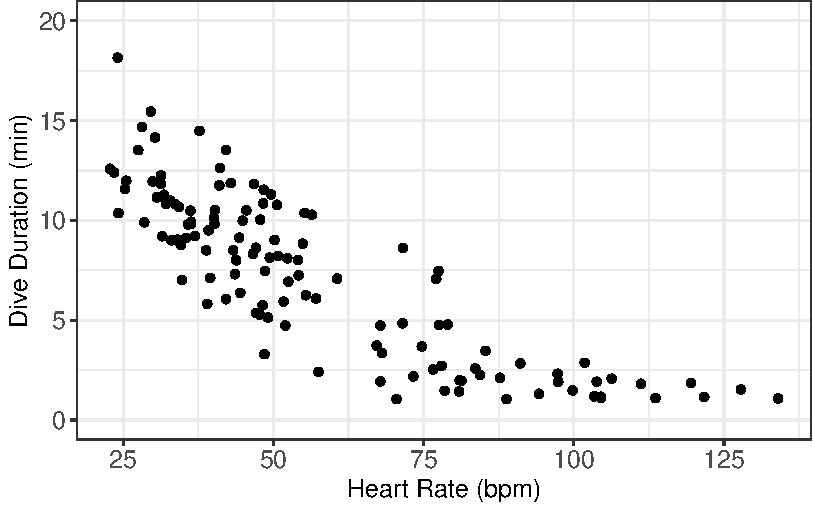
\includegraphics[width=0.7\textwidth,height=\textheight]{activity4-diving-penguins-key_files/figure-pdf/draw-line-1.pdf}

}

\end{figure}

\key{You just visually fit a linear regression by eye. There are some interesting perceptual properties of fitting lines through a set of points that we will not get into. Your line is likely not the same as your group member's but they might all have similarities.}

\hypertarget{finding-the-best-regression-line}{%
\subsection{Finding the ``Best'' Regression
Line}\label{finding-the-best-regression-line}}

Your regression line will be different from my regression line and from
other people in our class. There may be similarities, but no one will
draw the exact same line! So, how then do we decide what line is the
``best''?

In statistics we use a method called ``least squares.'' The idea is that
we minimize the sum of the squared distances between each point and the
line. That's a mouthful! Let's visualize what this means.

\textbf{10. On your plot, draw the vertical distance between some of the
points and the line you drew.}

\key{These vertical lines between the observed dive duration (points) and the predicted dive duration (line) for that heart rate are called residuals.}

\vspace{0.5cm}

These vertical distances are how far off your estimated duration is from
what was actually seen in the data. These values are called
\textbf{residuals}. The least squares method finds the line that
minimizes the \emph{square} of these residuals.

\vspace{0.5cm}

\textbf{11. When you square small residuals what happens?} \emph{Hint:
What happens if you square a value between 0 and 1? What about a small
value greater than 1?}

\key{Squaring a small residual (between 0 and 1) will result in a value smaller than your residual. Squaring a smaller value larger than 1 still results in a relatively small number (e.g. $2^2$ = 4).}

\vspace{0.5cm}

\textbf{12. When you square large residuals what happens?}

\key{Squaring a large residual will blow the resulting value up (e.g. $8^2$ = 64).}

\vspace{0.5cm}

\hypertarget{obtaining-coefficient-estimates-from-r}{%
\subsection{\texorpdfstring{Obtaining Coefficient Estimates from
\texttt{R}}{Obtaining Coefficient Estimates from R}}\label{obtaining-coefficient-estimates-from-r}}

We will always use \texttt{R} to find the equation of the ``best''
regression line. Specifically, we will use the \texttt{lm()} function.
The \texttt{lm} stands for \emph{linear model} - the method we believe
best models the relationship between our two variables.

The code will always look something like:

\begin{verbatim}
name_of_lm <- lm(<Y-VARIABLE> ~ <X-VARIABLE>, 
                 data = <NAME OF DATASET>)
\end{verbatim}

In the context of these data, here is the code I used to find the
regression line:

\emph{Note: We named our linear regression model \texttt{diving\_lm}.}

\begin{Shaded}
\begin{Highlighting}[]
\NormalTok{diving\_lm }\OtherTok{\textless{}{-}} \FunctionTok{lm}\NormalTok{(Duration }\SpecialCharTok{\textasciitilde{}}\NormalTok{ Dive\_HeartRate,}
                \AttributeTok{data =}\NormalTok{ diving)}
\end{Highlighting}
\end{Shaded}

Once we've told \texttt{R} to find the regression line, we need to
obtain the estimated coefficients that go with the line! To do this, we
will use the \texttt{get\_regression\_table()} function from the
moderndive package.

\emph{Note: We can use this function on the linear regression model we
named above.}

\begin{Shaded}
\begin{Highlighting}[]
\FunctionTok{get\_regression\_table}\NormalTok{(diving\_lm)}
\end{Highlighting}
\end{Shaded}

\begin{verbatim}
# A tibble: 2 x 7
  term           estimate std_error statistic p_value lower_ci upper_ci
  <chr>             <dbl>     <dbl>     <dbl>   <dbl>    <dbl>    <dbl>
1 intercept        14.8       0.466      31.6       0   13.8     15.7  
2 Dive_HeartRate   -0.131     0.007     -17.6       0   -0.146   -0.116
\end{verbatim}

\textbf{13. Using the output from the \texttt{R} code above, write the
equation of the regression line. Note that we've used variable names in
the equation, not generic \(x\) and \(y\). And put a carat (``hat'')
over the \(y\)-variable name to emphasize that the line gives predicted
values of the \(y\) (response) variable.}

\vspace{0.25cm}

\key{$$\widehat{\text{Dive Duration}} = 14.758 + -0.131 \times \text{(Heart Rate)}$$}

\vspace{0.25cm}

Notation: The equation of the best fit line is written as
\(\hat{y} = b_0 + b_1 \times \text{(x)}\) where

\begin{itemize}
\tightlist
\item
  \(b_0\) is the intercept
\item
  \(b_1\) is the slope
\item
  \(x\) is a value of the explanatory variable
\item
  \(\hat{y}\) is the predicted value for the response variable
\end{itemize}

\textbf{14. Is the slope positive or negative? Explain how the sign of
the slope tells you about whether your data display a positive or a
negative association.}

\key{The observed slope $b_1=-0.131$ is negative which tells us the data display a negative association because the line will be decreasing from left to right.}

\vspace{0.5cm}

\fbox{\begin{minipage}{45em}
\textbf{\large{Key Idea}} \\
For a given data set, the signs (positive or negative) for the correlation coefficient and the slope of the regression line must be the same.
\end{minipage}
}

\hypertarget{interpreting-the-coefficients}{%
\subsection{Interpreting the
Coefficients}\label{interpreting-the-coefficients}}

Let's investigate what the slope means in the context of heart rate and
dive duration.

\textbf{15. Use the least squares regression line to predict the diving
duration for penguins with a heart rate of 75 beats per minute.}

\key{$\widehat{\text{Dive Duration}} = 14.758 + -0.131\times 75=4.933$}

\vspace{0.5cm}

\textbf{16. Use the least squares regression line to predict the diving
duration for penguins with a heart rate of 76 beats per minute.}

\key{$\widehat{\text{Dive Duration}} = 14.758 + -0.131\times 76=4.802$}

\vspace{0.5cm}

\textbf{17. By how much do your predictions in \#8 and \#9 differ? Does
this number look familiar? Explain.}

\key{$4.933-4.802=0.131$, notice this is the same value as our estimated slope ($b_1$).}

\vspace{0.5cm}

\textbf{18. These questions above were designed to help you interpret
the slope. Interpret the slope in context:}

\key{The slope of the regression line predicting dive duration based on heart rate is 0.131, meaning that for every 1 beat per minute increase in heart rate, the predicted dive duration (increases / decreases) by 0.131 minutes.}

\vspace{0.5cm}

\fbox{\begin{minipage}{45em}
\textbf{\large{Key Idea}} \\
The slope coefficient of a least squares regression model is interpreted as the predicted change in the mean response ($y$) variable for a one-unit change in the explanatory ($x$) variable. 
\end{minipage}
}

Let's investigate the meaning of the \(y\)-intercept in the context of
dive duration and heart rate.

\textbf{19. Use the least squares regression line to predict the diving
duration for a penguin with a heart rate of 0 beats per minute.}

\key{$\widehat{\text{Dive Duration}} = 14.758 + -0.131\times 0=14.758$}

\{A penguin with a heart rate of 0 bpm could theoretically dive for a
durration of 14.758 minutes. Seems strange, huh? See the notes about
extrapolation below!\}

\vspace{0.5cm}

\textbf{20. Your answer to \#12 should look familiar. What is this
value?}

\key{$14.758$, notice this is the same value as our estimated intercept ($b_0$).}

\vspace{0.5cm}

\fbox{\begin{minipage}{45em}
\textbf{\large{Key Idea}} \\
The y-intercept of a regression line is interpreted as the predicted value of the response variable when the explanatory variable has a value of zero.
\end{minipage}
}

\hypertarget{be-cautious}{%
\subsection{Be cautious!}\label{be-cautious}}

While we can make predictions using our least squares regression line,
we should always be wary of extrapolation in interpreting the intercept
or other values outside the original data range.

\fbox{\begin{minipage}{45em}
\textbf{\large{Key Idea}} \\
Predicting values for the response variable for values of the explanatory variable that are outside of the range of the original data is known as ***extrapolation*** and can give very misleading predictions.
\end{minipage}
}

\begin{figure}

{\centering 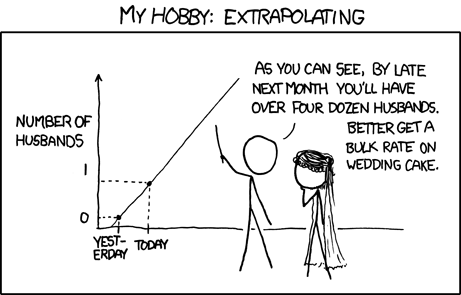
\includegraphics[width=0.5\textwidth,height=\textheight]{extrapolating.png}

}

\end{figure}

\textbf{21. What was the lowest value of heart rate observed in these
data?}

\key{The lowest heart rate shown on the graph is about 20 (22.8 to be exact).}

\vspace{0.5cm}

\textbf{22. What heart rates do you believe would be an extrapolation?}

\key{Any heart rate below the minimum of about 20 and above a heart rate of about 135 would be extrapolation because we do not have data on the duration of a dive outside of this range.}

\vspace{0.5cm}

\hypertarget{coefficient-of-determination}{%
\subsection{Coefficient of
Determination}\label{coefficient-of-determination}}

A quantity related to the correlation coefficient (r) is called the
coefficient of determination or R-squared (\(R^2\)). The coefficient of
determination (\(R^2\)) is the percentage of total observed variation in
the response variable that is accounted for by changes (variability) in
the explanatory variable.

Keep in mind that \(R^2\), like correlation, requires that the
relationship between the explanatory and response variables is linear!

\(R^2\) values are reported as proportions, but can also be thought of
as a percent. Values close to 1 or 100\% indicate that the explanatory
variable is able to explain a large portion of the variability in the
response.

We calculate \(R^2\) by squaring the correlation (r).

\textbf{23. Calculate the coefficient of determination (\(R^2\)) for the
relationship between heart rate and dive duration.} \emph{Hint: Look
back at question 5.}

\key{$R^2 = (-0.84)^2=0.7056$.}

\vspace{0.5cm}

\textbf{24. Complete the following statement to interpret what this
value means in the context of the data:}

\textbackslash key\{The coefficient of determination is 70.56\%, this
means that 70.56\% of the variation in penguin's dive duration is
attributable to changes in their heart rate\}.

\hypertarget{recall-the-context-of-todays-exploration}{%
\subsection{Recall the Context of Today's
Exploration}\label{recall-the-context-of-todays-exploration}}

Let's remember what the purpose of this study was. For the penguin
study, researchers equipped emperor penguins with devices that record
their heart rates during dives. The data we analyzed contained Dive
Heart Rate (beats per minute), the Duration (minutes) of dives, and
other related variables. \emph{These researchers were interested in
studying if there was evidence of an association between a penguin's
dive heart rate and the duration of their dive?}

\vspace{0.5cm}

\textbf{25. Write out the null and alternative hypothesis in words.}

\key{Null: There is no association between a penguin's dive heart rate and the duration of their drive.}

\key{Alternative: There is an association between a penguin's dive heart rate and the duration of their drive.}

\vspace{0.5cm}

\textbf{26. Using the research question, rewrite the hypotheses using
notation. Use the slope as the summary measure.} \emph{Hint: What is the
symbol for the population slope?}

\key{$H_O: \beta_1 = 0$}

\key{$H_O: \beta_1 \ne 0$}

\vspace{0.5cm}

\hypertarget{inference-for-the-slope-coefficient}{%
\subsection{Inference for the Slope
Coefficient}\label{inference-for-the-slope-coefficient}}

\textbf{27. Based on the slope coefficient you reported in question 14,
do you think there is convincing evidence of an association between a
penguin's heart rate and the duration of their dive?}

\key{The estimated slope from the observed data is, $b_1=-0.131$. This value is not zero and indicates a negative trend, but it is not too far away from 0 so it is hard to say.}

\vspace{0.5cm}

\hypertarget{hypothesis-testing}{%
\section{Hypothesis Testing}\label{hypothesis-testing}}

In a hypothesis test we are interested in comparing two things:

\begin{itemize}
\tightlist
\item
  what we observed in our data (our observed slope)
\item
  what would have happened if the null hypothesis was true
\end{itemize}

In order to compare what we saw in this study to what would have
happened if the null hypothesis was true, we need to generate a
distribution of slopes that we would have expected to see if the null
was true. This is called our \textbf{null distribution}. We then see
where our observed slope falls on that distribution.

If our observed statistic falls in the middle of the distribution, then
it is fairly likely to happen if the null is true. However, if our
observed statistic falls in the tails of the distribution, then it is
unlikely to happen if the null is true.

\hypertarget{simulation-based-methods}{%
\subsection{Simulation-Based Methods}\label{simulation-based-methods}}

Similar to what we talked about with confidence intervals and
bootstrapping, a null distribution is also a \emph{sampling
distribution}. It is, however, a special type of sampling distribution.
It is a distribution of sample statistics that could have been observed
\textbf{if the null hypothesis was true}.

Much like we used a bootstrap or a \(t\)-distribution to approximate the
true sampling distribution, there are two ways to approximate the true
null distribution:

\begin{enumerate}
\def\labelenumi{(\arabic{enumi})}
\item
  using simulation or
\item
  using a \(t\)-distribution.
\end{enumerate}

In this activity we will focus on option 1, but in the lab we will focus
on option 2.

\hypertarget{simulating-what-could-have-happened-under-the-null-hypothesis}{%
\subsubsection{Simulating what could have happened under the null
hypothesis}\label{simulating-what-could-have-happened-under-the-null-hypothesis}}

Let's start by thinking about how one simulation would be created on the
null distribution using cards.

\begin{itemize}
\tightlist
\item
  Step 1: Write each penguin's heart rate and dive duration on 125 cards
  - (\(x\),\(y\)) pairs.
\end{itemize}

\vspace{0.5}

\begin{itemize}
\tightlist
\item
  Step 2: Assume the null hypothesis is true - rip apart the pairs and
  make a pile of heart rate values and a pile of dive duration values.
\end{itemize}

\vspace{0.5cm}

\begin{itemize}
\tightlist
\item
  Step 3: Generate a new sample - match a randomly drawn heart rate with
  a randomly drawn dive duration until all cards have a random match
  (this is called permuting).
\end{itemize}

\vspace{0.5cm}

\begin{itemize}
\tightlist
\item
  Step 4: Calculate the statistic of interest - calculate the slope from
  the linear regression line fit on the randomly matched pairs of heart
  rate and dive duration.
\end{itemize}

\vspace{0.5cm}

\begin{itemize}
\tightlist
\item
  Step 5: Repeat and plot the statistic of interest from each random
  permutation on a dot-plot to create your null distribution.
\end{itemize}

\vspace{0.5cm}

\hypertarget{how-do-we-do-this-in-r}{%
\subsubsection{\texorpdfstring{How do we do this in
\texttt{R}?}{How do we do this in R?}}\label{how-do-we-do-this-in-r}}

We will use the \textbf{infer} package to help us simulate what could
have happened if the null was true. The layout for the code looks
similar to what you saw in last week's activity, so let's try and fill
in what is missing.

\begin{Shaded}
\begin{Highlighting}[]
\NormalTok{diving }\SpecialCharTok{\%\textgreater{}\%} 
  \FunctionTok{specify}\NormalTok{(}\AttributeTok{response =}\NormalTok{ \_\_\_\_\_\_\_\_\_\_\_, }
          \AttributeTok{explanatory =}\NormalTok{  \_\_\_\_\_\_\_\_\_\_\_) }\SpecialCharTok{\%\textgreater{}\%} 
  \FunctionTok{hypothesise}\NormalTok{(}\AttributeTok{null =} \StringTok{"independence"}\NormalTok{) }\SpecialCharTok{\%\textgreater{}\%} 
  \FunctionTok{generate}\NormalTok{(}\AttributeTok{reps =}\NormalTok{  \_\_\_\_\_\_\_\_\_\_\_, }
           \AttributeTok{type =}\NormalTok{  \_\_\_\_\_\_\_\_\_\_\_) }\SpecialCharTok{\%\textgreater{}\%} 
  \FunctionTok{calculate}\NormalTok{(}\AttributeTok{stat =} \StringTok{" \_\_\_\_\_\_\_\_\_\_\_"}\NormalTok{)}
\end{Highlighting}
\end{Shaded}

\textbf{28. What inputs should be entered for each of the following to
create the simulation to test regression slope?}

\vspace{.5 mm}

\begin{itemize}
\tightlist
\item
  Response variable (choose \texttt{Duration} or
  \texttt{Dive\_HeartRate}): \key{Duration}
\end{itemize}

\vspace{0.2in}

\begin{itemize}
\tightlist
\item
  Explanatory variable (choose \texttt{Duration} or
  \texttt{Dive\_HeartRate}): \key{$\text{Dive}\_\text{HeartRate}$}
\end{itemize}

\vspace{0.2in}

\begin{itemize}
\tightlist
\item
  Number of repetitions: \key{N permutations - we will do 5000.}
\end{itemize}

\vspace{.2in}

\begin{itemize}
\tightlist
\item
  Type of method to use when generating new samples (choose
  \texttt{"permute"} or \texttt{"bootstrap"}): \key{"permute"}
\end{itemize}

\vspace{0.2cm}

\begin{itemize}
\tightlist
\item
  Summary measure (choose \texttt{"slope"} or \texttt{"correlation"}):
  \key{"slope"}
\end{itemize}

\vspace{0.2in}

\textbf{29. Suppose we wanted to complete the simulation test using
correlation as the summary measure, instead of slope. Which input(s) in
\#4 would need to be changed to test for correlation? What input(s)
should you use instead?}

\key{Change the Summary measure input to "correlation".}

\vspace{0.5cm}

Here is a preview of what the output of this code looks like for 5000
permutations:

\emph{Note: We name the values in our null distribution (plotted in the
next histogram), \texttt{null\_dist}}

\begin{Shaded}
\begin{Highlighting}[]
\FunctionTok{head}\NormalTok{(null\_dist) }\SpecialCharTok{\%\textgreater{}\%}\NormalTok{ knitr}\SpecialCharTok{::}\FunctionTok{kable}\NormalTok{(}\AttributeTok{digits =} \DecValTok{3}\NormalTok{)}
\end{Highlighting}
\end{Shaded}

\begin{longtable}[]{@{}rr@{}}
\toprule()
replicate & stat \\
\midrule()
\endhead
1 & -0.003 \\
2 & -0.008 \\
3 & 0.002 \\
4 & 0.004 \\
5 & 0.003 \\
6 & 0.012 \\
\bottomrule()
\end{longtable}

\vspace{0.1in}

\textbf{30. What does the \texttt{replicate} column represent?}

\key{The replicate column represents one permutation of the observed data (replicate 1 = permutation 1, replicate 2 = permutation 2, etc.)}.

\vspace{0.5cm}

\textbf{31. What does the \texttt{stat} column represent?}

\key{The stat column is the calculated slope from the linear regression fit on that replicate/permutation of data.}

\vspace{0.5cm}

\hypertarget{visualizing-the-null-distribution}{%
\subsection{Visualizing the Null
Distribution}\label{visualizing-the-null-distribution}}

Below is a null distribution of slope statistics, generated using the
code you completed above. I chose to use 5000 reps, which might be
slightly different from what you chose.

\begin{figure}

{\centering 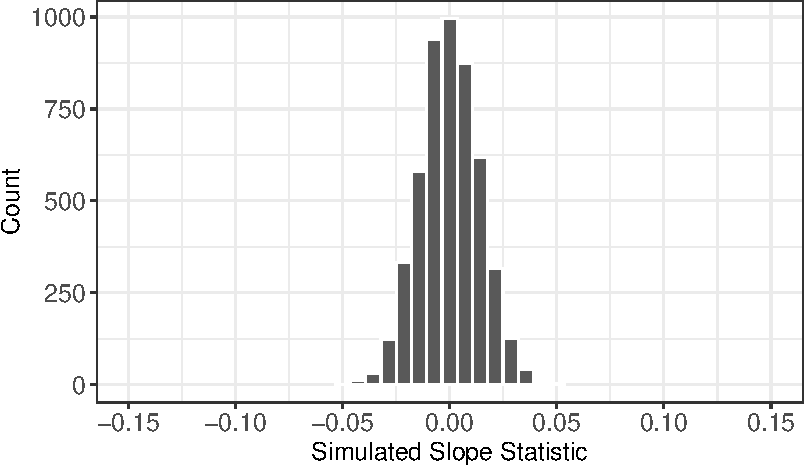
\includegraphics{activity4-diving-penguins-key_files/figure-pdf/null-viz-1.pdf}

}

\end{figure}

\vspace{0.2in}

\textbf{32. Why is the distribution centered at 0?}

\key{The null distribution is centered at 0 because it is simulated under the assumption there is no association between the heart rate and dive duration of a penguin.}

\vspace{1in}

\textbf{33. Mark where the observed slope lies on the distribution.}

\begin{figure}

{\centering 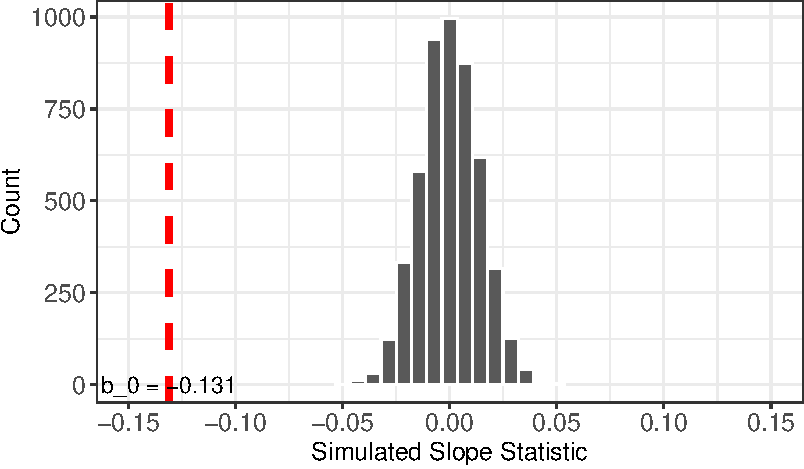
\includegraphics{activity4-diving-penguins-key_files/figure-pdf/null-viz2-1.pdf}

}

\end{figure}

\textbf{34. Shade or circle what area you will use to calculate the
p-value.}

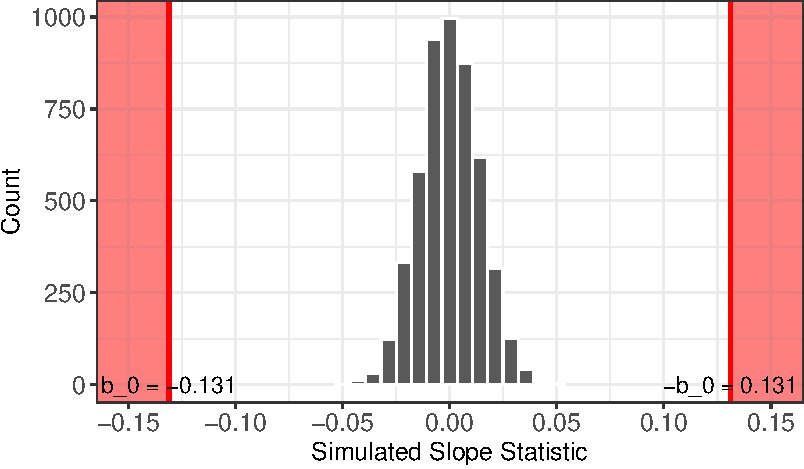
\includegraphics{activity4-diving-penguins-key_files/figure-pdf/unnamed-chunk-1-1.pdf}

\textbf{35. Estimate what p-value we will obtain from \texttt{R}.}

\key{Since none of our permutation samples resulted in an estimated slope as extreme as |-0.131|, I expect the p-value to be 0.}

\hypertarget{calculating-the-p-value}{%
\subsection{Calculating the p-value}\label{calculating-the-p-value}}

Since our distribution consists of 5000 slope statistics, we will need
to use \texttt{R} to find our p-value. To find a p-value, \texttt{R}
needs to first know what our observed statistic is. We can actually do
this using some of the code from before!

What I'm doing in the code below is:

\begin{itemize}
\tightlist
\item
  making a new object named \texttt{obs\_stat} that contains the number
  for the observed slope
\item
  using the \texttt{diving} data set
\item
  \texttt{specifying} what variables to use
\item
  \texttt{calclating} the statistic we are interested in
\end{itemize}

\emph{Note: we name this value in R, \texttt{obs\_slope}.}

\begin{Shaded}
\begin{Highlighting}[]
\NormalTok{obs\_slope }\OtherTok{\textless{}{-}}\NormalTok{ diving }\SpecialCharTok{\%\textgreater{}\%} 
  \FunctionTok{specify}\NormalTok{(}\AttributeTok{response =}\NormalTok{ Duration, }
          \AttributeTok{explanatory =}\NormalTok{ Dive\_HeartRate) }\SpecialCharTok{\%\textgreater{}\%} 
  \FunctionTok{calculate}\NormalTok{(}\AttributeTok{stat =} \StringTok{"slope"}\NormalTok{)}

\NormalTok{obs\_slope}
\end{Highlighting}
\end{Shaded}

\begin{verbatim}
Response: Duration (numeric)
Explanatory: Dive_HeartRate (numeric)
# A tibble: 1 x 1
    stat
   <dbl>
1 -0.131
\end{verbatim}

The next part is to compare this \texttt{obs\_stat} to the distribution
of shuffled slope statistics (stored in \texttt{null\_dist}).

\begin{Shaded}
\begin{Highlighting}[]
\FunctionTok{get\_p\_value}\NormalTok{(null\_dist, }
            \AttributeTok{obs\_stat =}\NormalTok{ \_\_\_\_\_\_\_\_\_\_, }
            \AttributeTok{direction =} \StringTok{"\_\_\_\_\_\_\_\_\_"}\NormalTok{)}
\end{Highlighting}
\end{Shaded}

\textbf{36. What inputs should be entered for each of the following to
calculate the p-value?}

\begin{itemize}
\tightlist
\item
  \texttt{obs\_stat\ =} \key{$\text{obs}\_\text{slope}$}
\end{itemize}

\vspace{.2cm}

\begin{itemize}
\tightlist
\item
  \texttt{direction\ =} (\texttt{"greater"}, \texttt{"less"}, or
  \texttt{"two-sided"}): \key{"two-sided"}
\end{itemize}

\vspace{.2cm}

Using your inputs, I obtained the p-value for our observed slope
statistic. The p-value is:

\begin{verbatim}
Warning: Please be cautious in reporting a p-value of 0. This result is an
approximation based on the number of `reps` chosen in the `generate()` step. See
`?get_p_value()` for more information.
\end{verbatim}

\begin{verbatim}
# A tibble: 1 x 1
  p_value
    <dbl>
1       0
\end{verbatim}

\vspace{0.2in}

\textbf{37. Why did I get a warning message from \texttt{R}? What does
the warning tell me?}

Warning: Please be cautious in reporting a p-value of 0. This result is
an approximation based on the number of \texttt{reps} chosen in the
\texttt{generate()} step. See \texttt{?get\_p\_value()} for more
information.

\key{The warning message from R is telling us to be cautious of reporting a p-value of 0 because our result is based on permutations and theortically one could possibly have had a slope as extreme as 0.131. When a p-value is "0", we say our p-value < 0.0001.}

\hypertarget{communicate-the-results-and-answer-the-research-question}{%
\subsection{Communicate the results and answer the research
question}\label{communicate-the-results-and-answer-the-research-question}}

\textbf{38. Based on the p-value and an \(\alpha = 0.05\), write a
conclusion in context of the problem.}

\key{p-value $< 0.0001 < 0.05 \implies$ Reject the null hypothesis.}

\key{We have evidence to conclude there is an association between a penguin's heart rate and their dive duration. Specifically, we have evidence to conclude the population slope between the heart rate and dive duration for all pegnuins is different from 0.}

\vspace{0.5cm}

\textbf{39. Based on the p-value you obtained for testing the slope,
what p-value do you think you would get if you tested the correlation
instead?} \emph{Hint: think about the relationship between slope and
correlation!}

\key{I would expect to see a p-value < 0.0001 since testing the slope is equivalent to testing the correlation. Recall, the correlation coefficient is used to calculate the slope.}

\vspace{0.5cm}

\hypertarget{connection-to-confidence-intervals}{%
\subsection{Connection to Confidence
Intervals}\label{connection-to-confidence-intervals}}

\textbf{40. If you were to make a 95\% confidence interval for the true
slope (\(\beta_1\)), would the interval contain 0? Why or why not?}

\key{No, since we rejected our null hypothesis based on a small p-value, our null value of 0 would not fall in the confidence interval and we would also reject based on the confidence interval.}

\vspace{0.5cm}

\newpage

\hypertarget{take-home-messages}{%
\subsubsection{Take-home messages}\label{take-home-messages}}

\begin{enumerate}
\def\labelenumi{\arabic{enumi}.}
\item
  To create one simulated sample on the null distribution when testing
  for a relationship between two quantitative variables, we separate the
  \(x\)-values from the \(y\)-values. We then shuffle the \(y\)-values
  and pair them with a new \(x\)-value. Once we have a new dataset, we
  find the regression line for the shuffled data and plot the slope or
  the correlation for the shuffled data.
\item
  To obtain a p-value for the observed slope we need to carry out the
  following steps:
\end{enumerate}

\begin{itemize}
\item
  obtain a distribution of statistics that could have happened if the
  null was true (null distribution)
\item
  locate the observed slope on the null distribution
\item
  count how many shuffled slopes are as large or larger than the
  observed slope
\item
  divide the number of slopes by the total number of reps used (e.g.,
  \(\frac{4}{1000}\))
\item
  multiply this by two, since we almost always have a two-sided
  alternative
\end{itemize}

\begin{enumerate}
\def\labelenumi{\arabic{enumi}.}
\setcounter{enumi}{2}
\tightlist
\item
  The p-value for a test for correlation should be approximately the
  same as the p-value for the test of slope. In the simulation test, we
  just change the statistic type from slope to correlation and use the
  appropriate sample statistic value.
\end{enumerate}



\end{document}
